\documentclass[11pt]{article}
\usepackage[margin = 1in]{geometry}
\usepackage{amsmath}
\usepackage{amssymb}
\usepackage{amsthm} % for proof environment
\usepackage{enumitem}
\usepackage{graphicx}
\usepackage{indentfirst}
\usepackage{caption}
\usepackage{lscape}
\usepackage{multirow}
\usepackage{array}
\usepackage{setspace}
\setlist{nolistsep}
\usepackage[round]{natbib}
\usepackage{accents}
\usepackage{caption}
\usepackage{subcaption}
\usepackage{xcolor}
\usepackage{setspace}
\onehalfspacing

\newcommand{\ubar}[1]{\underaccent{\bar}{#1}}
\newcommand{\p}{\prime}
\newcommand{\ev}{\mathbb{E}}
\newcommand{\lagr}{\mathcal{L}}
\newcommand{\inv}[1]{#1^{-1}}
\newcommand{\R}{{\rm I\!R}}
\newcommand{\U}{\mathcal{U}}
\renewcommand{\H}{\mathcal{H}}
\newcommand{\pderiv}[2]{\frac{\partial#1}{\partial #2}}
\newtheorem{proposition}{Proposition}

% Front matter
\title{Optimal Taxation with Heterogeneous Rates of Return}
\author{
    Nicholas Hoffman\\
    \and 
    Ali Shourideh\\
}

\begin{document}
\maketitle
\begin{abstract}
    We study optimal capital taxation in a model in which individuals are heterogeneous in the rates of return that they face. By offering individuals the choice between risk-free saving and risky investing, we capture the role that the government plays in ensuring that its most able entrepreneurs invest capital into their businesses. We allow the government to levy separate taxes on interest income from risk-free savings and on capital income earned by investing into private entrepreneurial enterprises. We derive properties of constrained-efficient allocations, and use a numerical model to illustrate the types of intertemporal wedges that may arise due to incentive constraints. The aim of this project is ultimately to compare the implementation of these wedges with a tax on capital income, and a tax on accumulated capital stock, or wealth. 
\end{abstract}

\section{Introduction} \label{intro}

Recent advances in data collection and economic modelling have given economists a strong understanding of the way in which the distribution of wealth in the United States has evolved to its current shape. We know that the fortunes of those on the top rung of the economic ladder are primarily composed of risky assets such as ownership of businesses and shares of stock. These fortunes are held by entrepreneurs, investors, and business owners--talented individuals who face a range of risks and rates of return in accumulating their wealth. Given these forces shaping the wealth distribution, however, it is less clear what sort of tax and transfer system is optimal to both satisfy the redistributive motives of the government and encourage investors to undertake risky projects with benefits that are beneficial to society. In order to study this question, we construct a model in which agents face differing rates of return, and a benevolent government levies taxes in order to satisfy utilitarian redistributive motives. 

The best way in which to tax the wealthy is a central focus of the current political debate. \cite{saez2019triumph} argue that, if one accounts for state, local, and sales taxes, the richest one hundredth of Americans pay a disproportionately small share of their income in taxes. Saez and Zucman attribute this regressive feature of the ex-post tax system to the treatment of capital income: owners of capital, they argue, are able to control the timing, amount, and even location of their income in a way that laborers are not. As a solution, they propose a tax on wealth directly, which they argue is more difficult to move or conceal. Critics of this approach note that such a tax discourages the type of risky investment that has long been the engine of economic growth. 

The Dynamic Public Finance literature, which began with the seminal work of \cite{mirrlees1971exploration}, offers us a way in which to weigh these concerns in implementing optimal capital taxation. What distinguishes this literature from prior work in optimal taxation (``Ramsey'' taxation) is that no exogenous restrictions are imposed on the tax schedule. Instead, the government can implement any type of tax that it wishes, subject to revenue requirements and endogenous informational frictions. Given the nonlinear tax schedules and informational frictions present in reality, we view this as an intuitively appealing setting in which to study capital taxation. 

A canonical result in the Ramsey literature, in which the government seeks to raise its revenue using the most non-distortionary linear taxes possible, is that the tax on capital should be set to zero.\footnote{See for instance \cite{atkinson1976design}, \cite{chamley1986optimal}, and \cite{judd1982redistributive}.} Perhaps the simplest reasoning behind this result is that the supply of capital is highly elastic, and any distortions introduced to the savings decisions of agents in the economy will decrease the future capital stock. In the presence of informational frictions, by contrast, it is often the case that capital taxes are nonnegative at the optimum.\footnote{\cite{golosov2003optimal} shows this result in a general setting.} In this case, the government taxes capital in order to prevent agents from self-insuring against idiosyncratic income shocks, ensuring that they will continue to exert labor effort. In most cases, however, these results arise in environments wherein even the wealthiest agents earn the bulk of their income in the labor market, and everyone saves at a common, risk-free rate. We investigate whether the optimality of nonnegative intertemoporal wedges remains when individuals face risk to their rates of return, and when the primary way in which wealthy agents earn income is through returns to capital--as is the case in reality. 

Given these wedges, we then turn to implementation in a competitive, dynamic economy. Studying implementations provides further motivation for allowing rates of return to be heterogeneous across the population. If all assets earn a constant rate, then there is an equivalence between taxing wealth and taxing capital income, and to a certain extent, either can be used to appropriately discourage savings. With different rates of return, however, this equivalence is lost, and taxes on capital income and wealth have fundamentally different impacts on behavior, and consequently, on government revenues. For this reason, a setting with heterogeneous and stochastic rates of return is an appropriate context for studying the different impacts of these tax schemes. 

We also consider this work a step in studying optimal taxation in the face of plausible processes for wealth accumulation. A number of different augmentations have been introduced to the workhorse heterogeneous models of \cite{aiyagari1994uninsured} and \cite{huggett1996wealth} in order to generate long-run distributions of wealth that match their empirical counterparts. Examples of such augmentations include \cite{quadrini2000entrepreneurship}, \cite{hubmer2016historical}, and \cite{benhabib2019wealth}, all of which produce long-run distributions of wealth more in line with the data. The widespread use of augmentations such as these demands a more thorough understanding of optimal taxation in a setting where agents face differing returns to saving. Our goal is to begin to build such an understanding: though at times we refer to agents who save capital in risky vehicles as ``entrepreneurs,'' our results apply to any setting in which agents can choose a portfolio of investments of varying risk and return. 

We proceed as follows. Section \ref{lit_rev} reviews the progress made in the literature around this topic to date, and highlights precisely how we aim to expand on these findings. In section \ref{two_pd}, we present a two-period version of our model, in which establish results on optimal intertemporal (savings) wedges. Section \ref{dyn_mod} extends our model to be fully dynamic, lasting for \( T > 2 \) periods. In this context, we aim to study how the optimal \textit{wedges} derived in section \ref{two_pd} translate into optimal \textit{taxes} in a competitive equilibrium under various tax regimes. Section \ref{conc} concludes. 

\section{Literature Review} \label{lit_rev}

Our study builds primarily upon a long line of research on optimal taxation. \cite{mirrlees1971exploration} introduced the canonical model, a static economy in which agents are privately informed of their own ability to turn labor effort into output. In contrast to prior literature, Mirrlees allowed the government to choose nonlinear tax schedules, provided that they incentivized each type to exert its allocated effort. Nevertheless, in his numerical examples, he found that the optimal labor income tax schedule was approximately linear over most of the distribution of productivities, and zero at the top and bottom. Following \cite{mirrlees1971exploration}, \cite{diamond1998optimal} and \cite{saez2001using} demonstrated, using empirically plausible preferences and distributions of ability, that while the optimal tax schedule may in fact be quite nonlinear, it is increasing in income, or progressive, over most of the distribution of ability.

\cite{golosov2003optimal}, \cite{kocherlakota2005zero}, and \cite{albanesi2006dynamic} extend this approach to dynamic economies, in which agents' skills evolve stochastically over time and risk-free savings is the only vehicle for self-insurance. \cite{golosov2003optimal} derive one of the key results in this literature: they demonstrate that for a wide class of specifications for the risk that agents face, the optimal tax system distorts their intertemporal consumption-savings decision, discouraging them from carrying too many assets into each period. \cite{kocherlakota2005zero} shows that this result holds in an economy subject to aggregate shocks. He also shows that the intertemporal wedge can be implemented by a tax system that is nonlinear in capital gains and linear in current wealth, and that in such a system, the tax on wealth is zero in the aggregate and raises no revenue. \cite{albanesi2006dynamic} construct a dynamic economy in which agents are subject to idiosyncratic shocks to their disutility of labor, and show that optimal allocations can be implemented using a simple tax schedule conditioned on wealth and current labor income. 

One common feature of these three papers is that the intertemporal rate of return on savings is constant across individuals, even if it may vary over time. Such a process of accumulation, however, fails to capture the way in which wealth is built in reality. \cite{benhabib2011distribution} show that the main    driver the thick tails in the wealth distribution-- such as those in the US data--is variation in individual rates of return. To see why this is the case, consider two favorable shocks to an agent: one affects his income, and the other affects the rate of return. The shock to income allows him to save more, increasing his wealth additively. The shock to his rate of return, however, \textit{multiplies} his wealth. It is this second type of shock that fills in the thick upper tail in the stationary distribution of wealth--particularly if an agent has the potential to realize several such favorable shocks consecutively.

Because variable rates of return can help models capture the thick tail in the empirical wealth distribution, a more recent strand of literature has attempted to characterize optimal taxation in settings where agents earn heterogeneous returns. \cite{phelan2019differential} considers a framework in which agents can hold a number of different assets, and the government is able to tax income from these assets according to different schedules. He finds that the tax on income from risky capital is constant throughout the population, and dependent only on the degree to which information is private, rather than individual productivities. In our model, the optimal tax on risky investment income does depend on the individual's idiosyncratic rate of return, or type. \cite{phelan2019business}, meanwhile, studies optimal wealth, labor, and capital income taxation in a context similar to ours, in which business owners' returns evolve according to a law of motion that depends upon their history of effort, as well as a random drift. Where our approaches differ is in the forces that generate disparate returns: agents in \cite{phelan2019business} have utility over consumption and leisure, and earn higher returns by investing more \textit{effort} over time. Our model, meanwhile, abstracts away from this mechanism, instead treating agent's average returns as an intrinsic characteristic, and allocating to entrepreneurs the investment of capital rather than effort.   

This paper begins by expanding the model of \cite{shourideh2014optimal}, in which agents are subject to both ex-ante and ex-post heterogeneity in the returns to their entrepreneurial investments. In this environment, where type, investment, and ex-post shocks are all unobservable, the optimal wedges for both risky investment and risk-free savings are increasing in type \( \theta \). We build upon this work in two ways. We add new sources of uncertainty in returns, and by doing so, impose additional constraints that the government must satisfy in order to incentivize truthful reporting. While the added informational frictions complicate the model, we show that they constrain the government in such a way as to allow us to incorporate a distribution for ability with wider support. In addition, we explicitly compare implementing the tax system with wealth and capital income taxes separately, and in doing so, aim to shed light on whether a tax on capital ought to depend on an agent's entire accumulated stock of assets, or just his most recent realized return. 

\section{Two-Period Economy} \label{two_pd}

Our model is most closely related to that in \cite{shourideh2014optimal}. Although the full model contains \( T\le\infty \) periods, for expositional purposes, we begin with a two-period version of the model, in which a number of results on optimal taxation in the full model can be shown. 

\subsection{Model} \label{model}

The economy is populated by a continuum of agents, indexed by \( i\in[0,1] \). Each agent has a privately-known type \( \theta\in\Theta=[\ubar{\theta},\bar{\theta}] \), distributed according to the C.D.F \( F(\theta) \). Time is discrete, and is given by \( t\in\{0,1\} \). Agents derive utility from consumption and discount the future at rate \( \beta \).
where \( c_t \) denotes consumption at time \( t \). All agents are endowed with initial wealth \( w \), which they allocate at \( t = 0 \) between consumption and savings. There are two assets in which agents may save for future consumption: risk-free savings bonds \( b \), and investment into their private entrepreneurial production technology \( k \). The price of the risk-free bond is normalized to one, and its return given by \( R > 0 \). If an agent of type \( \theta \) invests \( k \) into his entrepreneurial technology, his production at \( t = 1 \) is as follows:
\begin{equation}
    y = \begin{cases}
        \theta k \varepsilon & \text{with probability }\alpha \\
        0 & \text{with probability }1 - \alpha
    \end{cases}
\end{equation}
\( \varepsilon \) is an idiosyncratic shock to productivity, drawn from a distribution with C.D.F. \( H(\varepsilon) \). In particular, we assume that \( \varepsilon\sim\Gamma\left( \gamma,\inv{\gamma} \right) \). We define the distribution of second-period output, conditional on type \( \theta \) and investment \( k \) as 
\begin{equation}
    G\left( y|\theta,k \right) = H\left( \frac{y}{\theta k} \right)
\end{equation}

The government levies a tax on capital income, and is able to differentiate between income from risk-free saving and risky investment. Thus, the tax function has the form \( T(y,Rb) \), and the partial derivatives \( T_1 \) and \( T_2 \) give the marginal tax rates on the two types of investment income. The government is unable, however, to observe type \( \theta \), investment \( k \), or shock \( \varepsilon \). As noted in \cite{mirrlees1971exploration}, the government can be equivalently characterized as a benevolent social planner, who collects reports from agents on their type \( \theta \) and income \( y \), and allocates first-period consumption and investment \( \left( c_0(\theta),k(\theta) \right) \) and second-period consumption \( c_1(\theta,y) \). Henceforth, we use the terms ``government'' and ``planner'' interchangeably. For ease of exposition, we redefine the second-period allocations in terms of the shock \( \varepsilon \), rather than income \( y \): we define \( c_1(\theta,y) = c_1(\theta,\theta k\left( \theta \right) \varepsilon) \equiv c_1(\theta, \varepsilon) \).  

The planner's objective, then, is to maximize
\begin{equation}
    \int_{\ubar{\theta}}^{\bar{\theta}}\U(\theta)f(\theta)d\theta \label{plan_obj}
\end{equation}
where 
\begin{equation}
    \U(\theta) = u\left( c_0(\theta) \right) + \beta\left( \alpha\int_{0}^{\infty}u\left( c_1(\theta,\varepsilon) \right)dH(\varepsilon) + (1 - \alpha)u\left( c_1(\theta,0) \right)\right) \label{pkc}
\end{equation}
by choosing allocations \( \left( c_0(\theta),k(\theta) ,c_1(\theta,y) \right)\) for \( \theta\in\Theta \) and \( y\in\R_+ \). Throughout this paper, we assume that \( u(c) = \log(c) \). An allocation is said to be \textit{feasible} if it satisfies the resource constraints for \( t=0,1 \):
\begin{align}
    \int_{\ubar{\theta}}^{\bar{\theta}} \left[ c_0(\theta) + k(\theta) \right]f(\theta)d\theta &\le w \label{rc0} \\
    \alpha\int_{\ubar{\theta}}^{\bar{\theta}}\int_{0}^{\infty}\left[ \theta k(\theta)\varepsilon - c_1(\theta,\varepsilon) \right]h(\varepsilon)d\varepsilon f(\theta)d\theta + (1-\alpha)\int_{\ubar{\theta}}^{\bar{\theta}}c_1(\theta,0)f(\theta)d\theta &\le 0 \label{rc1}
\end{align}

Additionally, because the planner cannot observe \( \theta \) or \( k \), she must choose allocations that are \textit{incentive compatible}. Formally, the incentive constraints are formulated as follows: \( \forall \theta\in\Theta \),
\begin{equation}
    \theta, k(\theta)\in\arg\max_{\hat{\theta},\hat{k}}u\left( c_0(\hat{\theta}) + k(\hat{\theta}) - \hat{k} \right) + \beta\left( \alpha\int_{0}^{\infty}c_1(\hat{\theta},y)dH\left( \frac{y}{\theta \hat{k}} \right) + (1 - \alpha)u\left( c_1\left( \theta,0 \right) \right) \right) \label{ics}
\end{equation}
Note that because both type \( \theta \) and investment \( k \) are private information, (\ref{ics}) contains a double continuum of constraints. In order to impose these constraints in the planner's problem we employ the first-order approach, following \cite{jewitt1988justifying}. The constraints in (\ref{ics}) can be equivalently stated as follows:
\begin{align}
    u^\p\left( c_0(\theta) \right) &= \beta\alpha\int_{0}^{\infty}u\left( c_1\left( \theta,\varepsilon \right) \right)\frac{1}{k(\theta)}\left( -\varepsilon h^\p(\varepsilon) - h(\varepsilon) \right)d\varepsilon \label{ic_k} \\
    \U^\p(\theta) &= \frac{k(\theta)}{\theta}u^\p\left( c_0(\theta) \right) \label{ic_t}
\end{align}
Justification for this formulation can be found in the appendix. The crucial step is to think of the planner as observing \( y \) and collecting reports on type \( \theta \). Then, under the presumption that the agent has truthfully reported his type and invested the recommended \( k\left( \theta \right) \), the planner imputes a value for the agent's shock. Thus, if an agent of type \( \theta \) reports type \( \hat{\theta} \) and invests \( \hat{k} \), the shock that the planner will impute is given by 
\[\tilde{\varepsilon} = \frac{\varepsilon \theta \hat{k}}{\hat{\theta} k\left( \hat{\theta} \right)}\]
The agent will then be allocated consumption \( c_1(\theta,\tilde{\varepsilon}) \). This transformation allows us to calculate the marginal benefit of investing additional \( \hat{k} \) in terms of its effect on the distribution of imputed \( \tilde{\varepsilon} \) values. 
 
The planner faces one additional constraint in formulating optimal allocations. As we will show, if \( R \) is the risk-free rate, then the planner finds it optimal to incentivize all types \( \theta > R \) to invest \( k(\theta)>0 \). The agents who do so will face risk, including the nonzero probability that their capital investment return will be zero. The planner must ensure that these types are not better off eating their entire first-period allotment \( c_0(\theta) + k(\theta) \), investing nothing (and thus producing \( y = 0 \) with certainty), and then claiming to have been unlucky. Formally, we require that \( \forall\theta\in\Theta \),
\begin{equation}
    \U(\theta)\geq \max_{\hat{\theta}} u\left( c_0(\hat{\theta}) + k(\hat{\theta}) \right) + \beta u\left( c_1(\hat{\theta},0) \right) \label{nolie}
\end{equation}
In order to simplify the double continuum of constraints in (\ref{nolie}) we make the following two assumptions, which will prove to be innocuous. The first is that if \( \theta > R \), \( \U^\p(\theta) > 0 \); that is, the utility from optimal allocations is increasing in \( \theta \). The second is that 
\begin{equation}
    \bar{\theta} = \arg \max_{\hat{\theta}} u\left( c_0(\hat{\theta}) + k(\hat{\theta}) \right) + \beta u\left( c_1(\hat{\theta},0) \right) 
\end{equation}
that is, if an agent plans on absconding with all of his allocated capital and claiming to have been unlucky, it is optimal for him to claim to be type \( \bar{\theta} \). With these assumptions in place, (\ref{nolie}) can be reduced to a single constraint:
\begin{equation}
    \U(R)\geq u\left( c_0(\bar{\theta}) + k(\bar{\theta}) \right) + \beta u\left( c_1(\bar{\theta},0) \right) \label{nolie1}
\end{equation}
Thus, the planner's problem is to maximize (\ref{plan_obj}) subject to (\ref{rc0}), (\ref{rc1}), (\ref{ic_k}), (\ref{ic_t}), and (\ref{nolie1}).

\subsection{Characterizing Optimal Allocations}

Recall that the government levies taxes on risky investment income and risk-free saving via the (possibly nonlinear) tax function \( T(y,Rb) \), with partial derivatives \( T_1 \equiv \tau_k \) and \( T_2\equiv\tau_b \). As we will show, while these derivatives are somewhat analogous to marginal tax rates, they are not exactly identical. Nevertheless, our first step in deriving optimal taxes will be to derive the optimal intertemporal wedges for investment and saving, defined respectively as follows:
\begin{align}
    \tau_k(\theta) &= 1 - \frac{u^\p\left( c_0(\theta) \right)}{\beta\theta\int u^\p\left( c_1(\theta,\varepsilon) \right)\varepsilon h(\varepsilon)d\varepsilon} \label{tau_k} \\
    \tau_b(\theta) &= 1 - \frac{u^\p\left( c_0(\theta) \right)}{\beta R\int u^\p\left( c_1(\theta,\varepsilon) \right) h(\varepsilon)d\varepsilon} \label{tau_b} 
\end{align}

% What can we say about optimal allocations?
A full, closed-form characterization of optimal allocations in this context cannot be solved for. Nevertheless, we can prove a few properties that optimal allocations must satisfy, which will be helpful in determining the above wedges at the optimum. The first is that for the agents who produce \( y>0 \), consumption in the second period is linear in the shock \( \varepsilon \):
%
\begin{proposition} \label{c1_lin}
    Second-period consumption \( c_1(\theta,\varepsilon) = \phi\left(\theta\right)+\vartheta\left(\theta\right)\varepsilon \); that is, \( c_1(\theta,\varepsilon) \) is linear in \( \varepsilon \).
\end{proposition}
%
The proof, which closely follows \cite{shourideh2014optimal}, can be found in the appendix. The linearity of \( c_1(\theta,\varepsilon) \) is a consequence of our assumptions on utility and the distribution of \( \varepsilon \), but the fact that consumption is increasing in income is invariant to these assumptions. Agents who invest capital into their private projects face risk, and because they are assumed to be risk-averse, they must be compensated with increased consumption in order to incentivize them to take on this risk. 

\subsubsection{A Discrete Analogue}

In order to gain further insights into the optimal allocations in this model, we formulate a discrete analogue to the continuous model of section \ref{model}. We allow the distribution for \( \varepsilon \) to have continuous support over the real line, and we assume that \( \varepsilon\sim\Gamma(\gamma, \inv{\gamma}) \), where \( \Gamma(a,b) \) indicates the Gamma distribution with shape \( a \) and scale \( b \). We assume log utility, and parametrize the problem as follows:
\begin{align*}
    \beta &= 0.95 & R &= 1.0 & w &= 1.2 \\
    \alpha &= 0.9 & \gamma &= 2.0
\end{align*}
We assume a discrete grid for income \( y\in Y=\{y_1,\dots,y_{N_y}\} \). Agents and the planner can choose any \( k\ge 0 \), which determines their probability mass function over \( Y \), denoted \( \Pr\left( y|\theta,k \right) \)\footnote{\( \Pr\left( y|\theta,k \right) \) incorporates the fact that \( y=0 \) with probability \( 1-\alpha \).}. Agents are of type \( \theta\in\Theta=\{\theta_1,\dots,\theta_{N_\theta}\} \), each with equal probability \( N_\theta^{-1} \). The economy is once again populated by a continuum of agents, and so the law of large numbers guarantees that the various probabilities in our model translate into proportions of the population; for example, a proportion \( N_\theta^{-1} \) of the population has a given type \( i \), and of those, \( \alpha \) will produce \( y>0 \), while \( 1-\alpha \) will produce zero. Because \( k \) can take any nonnegative value, we use a two-step procedure to compute the incentive constraints. First, for each pair \( \left( \theta,\hat{\theta } \right)\in\Theta \), we compute 
\[k^*(\theta,\hat{\theta}) = \arg\max_{\hat{k}}u\left( c_0\left( \hat{\theta} \right) + k\left( \hat{\theta} \right)-\hat{k} \right) + \beta \sum_{i=1}^{N_y}u\left( c_1\left( \hat{\theta},y \right) \right)\Pr\left(y|\theta,\hat{k} \right)\]
Thus, \( k^*\left( \theta,\hat{\theta} \right) \) gives the optimal investment for an agent of type \( \theta \) reporting type \( \hat{\theta} \). Then, we impose the \( N_\theta^2 \) incentive constraints, which require that \( \forall\theta, \hat{\theta}\in\Theta \),
\begin{equation}
    \U(\theta)\geq \left( c_0\left( \hat{\theta} \right) + k\left( \hat{\theta} \right)-k^*\left( \theta,\hat{\theta} \right) \right) + \beta \sum_{i=1}^{N_y}u\left( c_1\left( \hat{\theta},y \right) \right)\Pr\left(y|\theta,k^*\left( \theta,\hat{\theta} \right)\right)
\end{equation}
given the \( k^* \) values computed above. Additionally, we require that \( k^*\left( \theta,\theta \right) = k(\theta) \); that is, if an agent truthfully reports his type, he must find it optimal to invest the amount recommended to him by the planner. Finally, we impose (\ref{nolie1}): we assume that \( R<\theta_1 \), and thus all types invest \( k>0 \), and require that
\begin{equation}
    U(\theta_1)\ge u\left( c_0\left( \theta_{N_\theta} \right) + k\left( \theta_{N_\theta} \right) \right) + \beta u\left( c_1\left( \theta_{N_\theta},0 \right) \right) \label{nolie_disc}
\end{equation}
We solve for allocations \( \{c_0(\theta), k(\theta), c_1(\theta,y),c_1(\theta,0)\} \) for each \( \theta\in\Theta \) and \( y\in Y \). From the household's problem, we define the wedges as follows:
\begin{align*}
    \tau_k(\theta) &= \frac{u^\p(c_0(\theta))}{\beta\theta\alpha \sum_{i=1}^{N_y}u^\p(c_1(\theta,y))\frac{y}{k(\theta)}\Pr\left( y|\theta,k(\theta),y>0 \right)} \\
    \tau_b(\theta) &= \frac{u^\p(c_0(\theta))}{\beta\theta \sum_{i=1}^{N_y}u^\p(c_1(\theta,y))\Pr\left( y|\theta,k(\theta) \right)}
\end{align*}

Figure \ref{alloc_disc} shows the optimal allocations for a grid \( \Theta \) with ten equally spaced points between 0.8 and 3.0, and a grid \( Y \) of forty points between zero and fifteen. We construct the grid \( Y \) such that lower \( y \) values are clustered closer together; most income values will be towards the bottom of this range, so we construct the grid in this way in order to make the solution more accurate at these lower \( y \) values. Beginning with the upper left-hand panel, higher types are unsurprisingly allocated more investment in the first period. Accordingly, the upper right-hand panel shows that these types can expect higher capital incomes in the second period, with more weight in the right tail of the distribution. As demonstrated in the bottom panel, consumption in the second period \( c_1(\theta,y) \) is increasing in \( y \), as expected. Interestingly, though, the ordering of \( c_1(\theta,y) \) is not constant over the grid \( Y \). Instead, for each \( \theta_i \), there is an interval over the space of incomes \( Y \) where \( \theta_i \) is allocated the most consumption among all \( \theta \) values. This nonlinear feature of the consumption schedule is a result of the incentive constraints: given a reported type, the planner knows the range of \( y \) values into which the agent's income will most likely fall. Knowing this, she sets the consumption schedule for this \( \theta \) such that the agent is best off investing the allocated amount, and ending up in their designated range. If the agent invests less that \( k(\theta) \), they are likely to fall below this range of incomes, where their consumption schedule decreases rapidly. Meanwhile, if they invest more, their income will likely be higher, but the consumption schedule flattens out at these values such that the loss in first-period consumption necessitated by this higher investment leaves the agents worse off on net. 

\begin{figure}[!htbp]
    \centering
    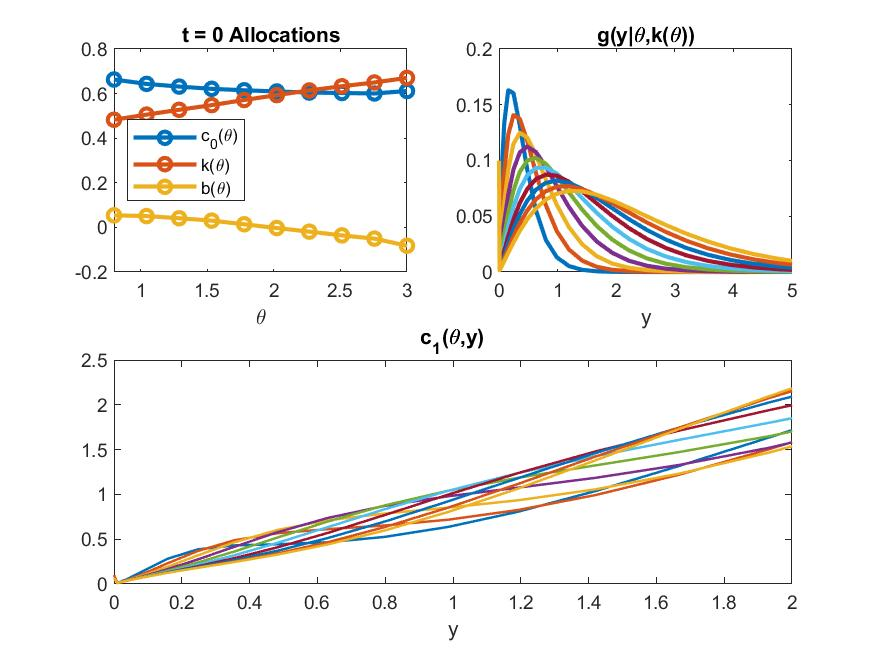
\includegraphics[scale = 0.4]{figures/allocations_10.jpg}
    \caption{Allocations in the Discrete Model}
    \label{alloc_disc}
\end{figure}

Figure \ref{wedge_disc}, meanwhile, shows the wedges at the optimum. In this example, capital income is actually subsidized at all levels, with \( \tau_k(\theta)<0 \) for all \( \theta\in\Theta \). These results primarily demonstrate the influence of the incentive constraints on the planner's problem. The lower \( \theta \) types, being less productive on average, would like to invest a greater proportion of their portfolio in a long position in the risk-free bond, and less into their risky capital, as compared to higher types. From the planner's perspective, however, allowing the lower productivity types to have such a portfolio is not compatible with her incentive constraints. Instead, the planner would rather the lower types have a higher proportion of risky assets, in order to discourage nearby types from misreporting their type. Accordingly, the planner sets the wedge on risk-free savings \( \tau_b \) at a high level, inversely proportional to \( \theta \). 

While the results in the discrete formulation are illustrative of the forces governing allocations in our model, these results are by no means definitive. Due to the maximization problem in the constraints, the algorithm is slow to converge even for low values of \( \theta \). As such, we are limited in the degree of ex-ante heterogeneity that we can capture. Furthermore, there is no guarantee that this problem converges to a global optimum. Indeed, the solution to this algorithm is a vector of allocations of dimension \( 2N_\theta + N_\theta N_y = 420 \), which makes searching over the entire space infeasible. As such, we are only guaranteed a local minimum, and further analytical results are needed to determine whether the allocations in Figure \ref{alloc_disc} can be improved upon. 

\begin{figure}[!htbp]
    \centering
    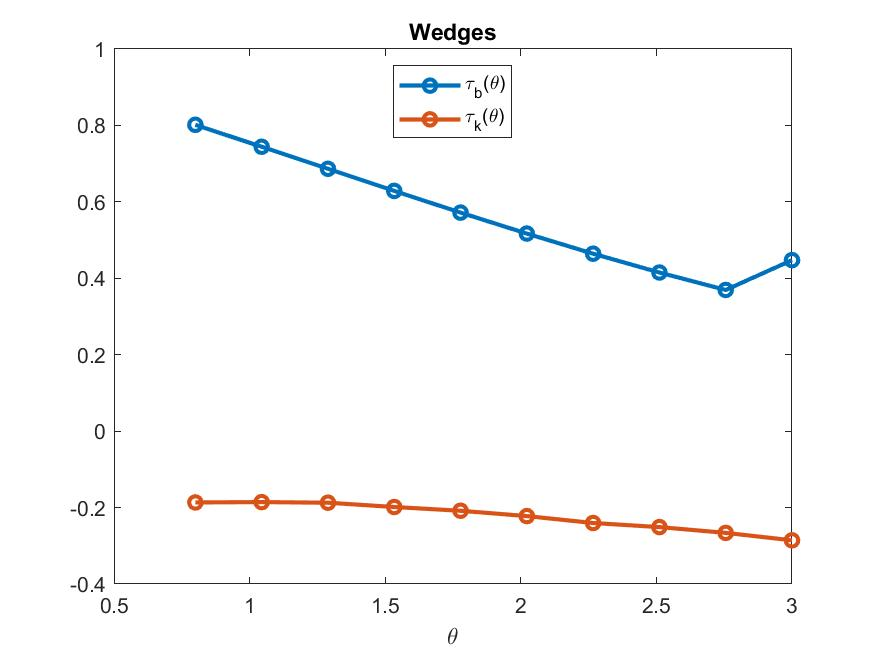
\includegraphics[scale=0.4]{figures/wedges_10.jpg}
    \caption{Wedges in the Discrete Model}
    \label{wedge_disc}
\end{figure}

\section{Full Dynamic Model} \label{dyn_mod}
\section{Conclusion} \label{conc}

We have studied optimal capital taxation a model in which agents can save in two assets: a risk-free instrument with common return, and a private entrepreneurial project, the return to which is subject to risk and heterogeneous throughout the population. We have shown that at the constrained efficient solution, consumption allocated to agents who invest capital is a linear function of the multiplicative shock \( \varepsilon \) to their return, with type-dependent slope and intercept. We also formulate a semi-discrete version of our model, and shown results for a specific parametrization. Under this specification, the planner finds it optimal to subsidize investment, and to set a high, positive wedge on interest income from risk-free saving. 

What remains is twofold: to carry out the analysis of optimal wedges in the two-period model, and to demonstrate how those wedges translate into taxes in the dynamic competitive version of the model. While our discrete formulation is useful for illustrating the ways in which the incentive constraints shape optimal allocations, the numerical results from this exercise do not hold in general. Instead, we will show that more features of optimal allocations can be derived analytically. 

Turning to the full dynamic model, we will study how the wedges derived in section \ref{two_pd} translate into taxes in a competitive equilibrium. We will construct a model in discrete time, in which agents make a (possibly infinite) series of consumption and savings decisions. In this economy, the government will tax either capital income or wealth according to a tax-and-transfer function \( T(\cdot) \). This function \textit{implements} the optimal distortions if it induces the agents to choose the constrained-efficient allocations. Finding these implementations will allow us to study whether the government is better off levying a tax on capital income, or on wealth. 

\bibliographystyle{named}
\bibliography{summer_paper}
\newpage
\section*{Appendix}
\renewcommand{\theequation}{A.\arabic{equation}}

\paragraph{First-Order Approach} 
The incentive constraints are 
\begin{equation}
    \theta, k(\theta)\in\arg\max_{\hat{\theta},\hat{k}}u\left( c_0(\hat{\theta}) + k(\hat{\theta}) - \hat{k} \right) + \beta\left( \alpha\int_{0}^{\infty}c_1(\hat{\theta},y)dH\left( \frac{y}{\theta \hat{k}} \right) + (1 - \alpha)u\left( c_1\left( \theta,0 \right) \right) \right) \label{eq:ics_app}
\end{equation}
These constraints can be stated equivalently as follows:
\begin{equation}
    \theta, k(\theta)\in\arg\max_{\hat{\theta},\hat{k}}u\left( c_0(\hat{\theta}) + k(\hat{\theta}) - \hat{k} \right) + \beta\left( \alpha\int_{0}^{\infty}c_1\left(\hat{\theta},\frac{\varepsilon\theta\hat{k}}{\hat{\theta}k\left( \hat{\theta}\right)} \right)dH\left( \varepsilon \right) + (1 - \alpha)u\left( c_1\left( \theta,0 \right) \right) \right) \label{eq:ics_alt}
\end{equation}
In the second formulation, the planner provides a schedule for consumption \( c_1(\theta,\varepsilon) \), and imputes the value of \( \varepsilon \) based on the agent's type and observed income, presuming that the agent has reported truthfully and invested the recommended amount. The first-order approach requires that the first-order conditions for \( \hat{\theta} \) and \( \hat{k} \) of (\ref{eq:ics_alt}) hold when evaluated at \( \hat{\theta}=\theta \) and \( \hat{k} = k(\theta) \). The first-order condition for (\ref{eq:ics_alt}) with respect to \( \hat{k} \) is 
\begin{equation}
    u^\p (c_0(\theta)) = \beta\alpha\int_{0}^{\infty}u\left( c_1\left( \theta,\varepsilon \right) \right) \frac{1}{k(\theta)}\left( -\varepsilon h^\p (\varepsilon)-h(\varepsilon) \right) \label{eq:icsk_app}
\end{equation}
as in (\ref{ic_k}). For \( \hat{\theta} \), we utilize the Envelope condition:
\begin{equation}
    \U(\theta) = \max_{\hat{\theta},\hat{k}}u\left( c_0(\hat{\theta}) + k(\hat{\theta}) - \hat{k} \right) + \beta\left( \alpha\int_{0}^{\infty}c_1(\hat{\theta},y)dH\left( \frac{y}{\theta \hat{k}} \right) + (1 - \alpha)u\left( c_1\left( \theta,0 \right) \right) \right) 
\end{equation}
and so by the Envelope theorem,
\begin{equation}
    \U^\p(\theta) = \frac{\partial}{\partial \hat{\theta}}\beta\alpha\int_{0}^{\infty}c_1(\hat{\theta},y)dH\left( \frac{y}{\theta \hat{k}} \right) \label{eq:env1}
\end{equation}
Because the right-hand side of (\ref{eq:env1}) is a function of the product \( \theta\hat{k} \), we make use of the following identity:
\begin{equation*}
    \frac{\partial}{\partial \theta}f(\theta k) = \frac{k}{\theta} \frac{\partial}{\partial k}f(\theta k)
\end{equation*}
Thus,
\begin{align*}
    \U^\p(\theta) &= \frac{k}{\hat{\theta}} \frac{\partial}{\partial k} \beta\alpha\int_{0}^{\infty}c_1(\hat{\theta},y)dH\left( \frac{y}{\theta \hat{k}} \right) \\
    &= \frac{k}{\theta}u^\p(c_0)
\end{align*}
where the final equality follows from the right-hand side of (\ref{eq:icsk_app}). This is the form in (\ref{ic_t}). \newpage

\paragraph{Proof of Proposition \ref{c1_lin}}
\begin{proof}
    Consider the planner's problem in (\ref{plan_obj}). The first-order conditions for \( c_1(\theta,\varepsilon) \) and \( c_1(\theta,0) \) give:
    \begin{align*}
        \lambda_{1}&=\beta u^{\prime}\left(c_{1}\left(\theta,0\right)\right)\eta \\
        \lambda_{1}&=\beta u^{\prime}\left(c_{1}\left(\theta,\varepsilon\right)\right)\eta+\beta u^{\prime}\left(c_{1}\left(\theta,\varepsilon\right)\right)\frac{1}{ k\left(\theta\right)}\left(-\varepsilon h^\p(\varepsilon)-h(\varepsilon)\right)\kappa f
    \end{align*}
    where \( \lambda_1 \) is the multiplier on the feasibility constraint in the first period (\ref{rc1}), and \( \eta(\theta) \) and \( \kappa(\theta) \) are the multipliers on (\ref{pkc}) and (\ref{ic_k}), respectively. Rearranging and combining, along with the assumption of log utility, gives
    \begin{align*}
        c_1(\theta,\varepsilon) &= c_{1}\left(\theta,0\right)+\kappa\beta\frac{1}{\lambda_{1} k}\frac{\left(-\varepsilon h^\p(\varepsilon)-h(\varepsilon)\right)}{h\left( \varepsilon \right)} \\
        &= c_{1}\left(\theta,0\right)+\kappa\beta\frac{1}{\lambda_{1}\gamma k}\left(\varepsilon-1\right) \\
        &\equiv \phi\left(\theta\right)+\vartheta\left(\theta\right)\varepsilon 
    \end{align*}
    where the penultimate inequality follows from the assumption that \( \varepsilon \) is drawn from a \( \Gamma\left( \gamma,\inv{\gamma} \right) \) distribution.
\end{proof}
\end{document}